\documentclass{beamer}
%\usetheme[secheader]{Lab2C}
\usetheme{Lab2C} % disable pgf drawing to speed up compilation in development
\usepackage{graphicx}
\usepackage{array}
\usepackage{subcaption}
\usepackage{listings}
\usepackage{color}
\usepackage{algorithmic}
\usepackage{amssymb}

\DeclareMathOperator{\Bern}{Bern}
\newcommand\independent{\protect\mathpalette{\protect\independenT}{\perp}}
\def\independenT#1#2{\mathrel{\rlap{$#1#2$}\mkern2mu{#1#2}}}

\definecolor{mygray}{rgb}{0.5,0.5,0.5}
\lstset{
numbers=left,
numbersep=5pt,
numberstyle=\tiny\color{mygray}
}

\newif\ifbeamer
\beamertrue
%\setbeamertemplate{footline}[frame number]
\logo{
\includegraphics[height=0.8cm]{ieee_logo.eps}}
\title[Error Rate of Stochastic Block Model with Symmetric Side Information]{On the Optimal Error Rate of Stochastic Block Model with Symmetric Side Information}
\author{Feng Zhao\inst{1} \and Jin Sima\inst{2}\and Shao-Lun Huang\inst{3}}
\institute{\inst{1}Dept. of Electronic Engineering, Tsinghua University
\and\inst{2}Department of Electrical Engineering, California Institute of Technology
	\and \inst{3}Tsinghua-Berkeley Shenzhen Institute, Tsinghua University 
	\\ \vskip 0.5cm ITW 2021}
\date{\today}
\begin{document}
\begin{frame}
	\titlepage
\end{frame}
%\section*{Outline}
\begin{frame}
	\tableofcontents
\end{frame}
\section{Background}
\subsection{Community Detection}
\begin{frame}{Community Detection}
	\begin{columns}
		\column{0.5\textwidth}
		\begin{figure}
			
\includegraphics[width=0.8\textwidth]{cd.png}
		\end{figure}
	\column{0.5\textwidth}
	Community Detection is inferring the group of vertices which are more
	densely connected in a graph
	\end{columns}
	\begin{columns}
		\column{0.33\textwidth}
		\begin{figure}
			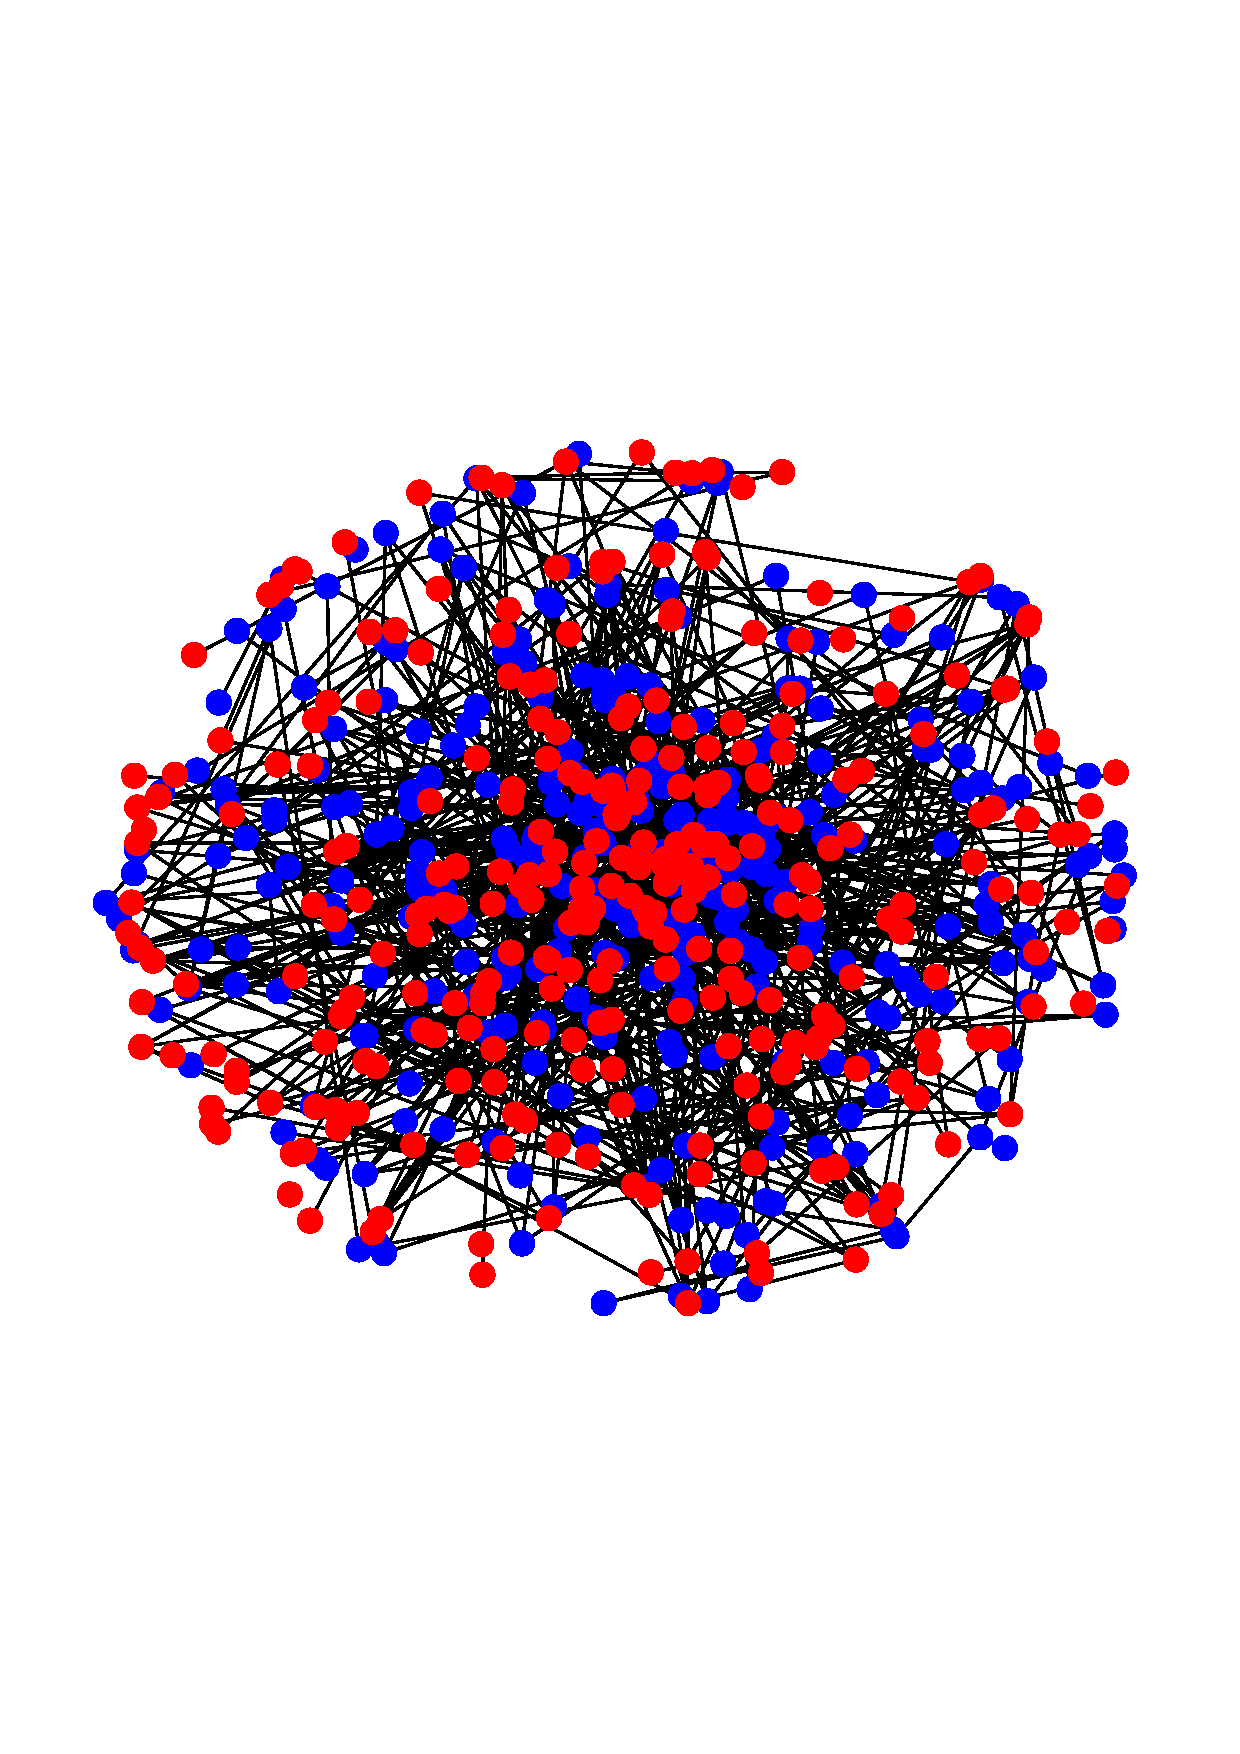
\includegraphics[width=\textwidth]{benno2t.pdf}
		\end{figure}
		\column{0.05\textwidth}
		$\Rightarrow$
		\column{0.5\textwidth}
		\begin{figure}
		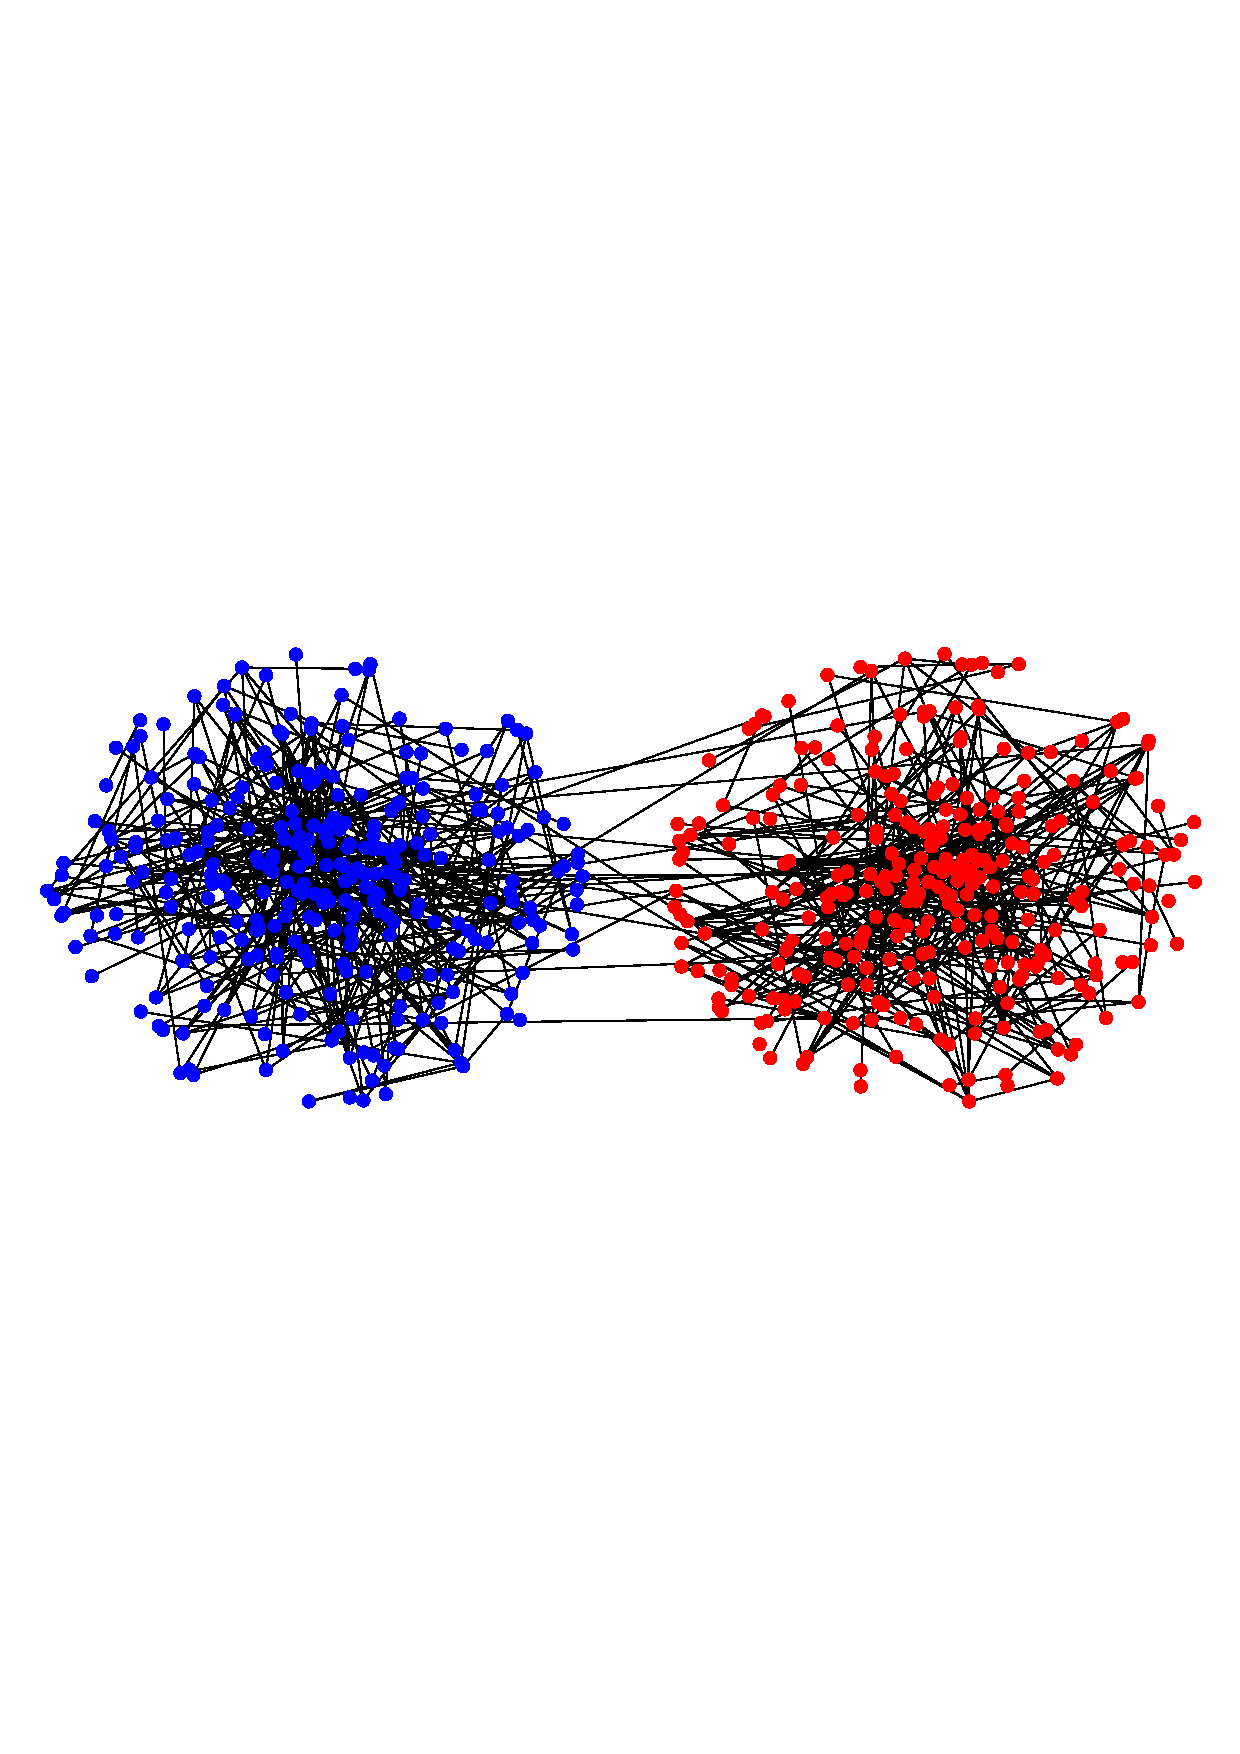
\includegraphics[width=\textwidth]{bennot.pdf}
		\end{figure}
	\end{columns}
\end{frame}
\begin{frame}{Community Detection with Side Information}
	\begin{columns}
		\column{0.5\textwidth}
	\begin{figure}
		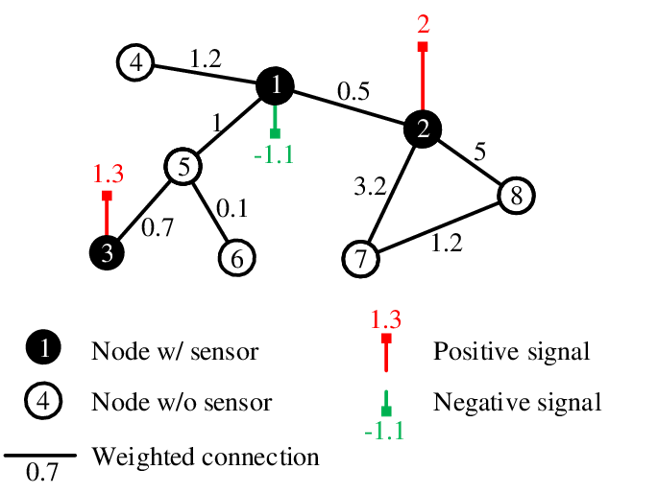
\includegraphics[width=0.8\textwidth]{si.png}
		\caption{\scriptsize Graph Model with Side Information}
	\end{figure}
	\column{0.5\textwidth}
	Incorporating side information in graph model
	can improve the performance of Community Detection
	\begin{block}{Objective}
		Investigate quantitatively how side information influences
		the detection error rate for a specific graph model
	\end{block}
	\end{columns}
\end{frame}
\subsection{Stochastic Block Model}
\begin{frame}{Binary Symmetric Stochastic Block Model}
	\begin{block}{Characteristics}
		\begin{itemize}
		\item a probabilistic model to generate random graph
		\item larger probability for the existence of edges within the same community
		\item smaller probability for the existence of edges between different communities
		\end{itemize}
		\end{block}
		\begin{columns}
			\column{0.33\textwidth}
				\begin{figure}
				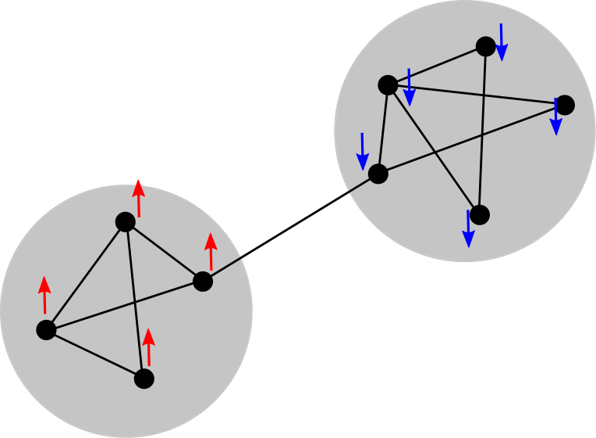
\includegraphics[width=\textwidth]{sbm.png}
			\end{figure}
		\column{0.67\textwidth}
		\quad$(G,Y)\sim \textrm{SSBM}(n, p, q)$
		\begin{itemize}
			\item $Y$: community labels
			\item $n$: the number of nodes
			\item $p$: probability of connecting within clusters
			\item $q$: probability of connecting across clusters
		\end{itemize}
		\end{columns}	
\end{frame}
\begin{frame}{Detection Algorithms and Recovery Metrics}
	\begin{description}
		\item[Observation] random graph $G$, generated by $\textrm{SSBM}(n,p,q)$;
		\item[Estimator] $\hat{Y}(G)$, an algorithm to recover node labels $Y$;
		\item[Error probability] $P_e=P(\hat{Y} \neq \pm Y)$
	\end{description}
	
	\begin{block}{Known Results [Abbe-Bandeira-Hall, 2014]}
		\begin{itemize}
		\item Community labels $Y$ are symmetric: half $+1$, half $-1$;
		\item $p = a\frac{ \log n}{n}, q = b \frac{ \log n}{n}$;
		$\sqrt{a} - \sqrt{b} > \sqrt{2}$
		\item $P_e \to 0$ as $n \to \infty$.
		\end{itemize}
	\end{block}
	\begin{block}{Problem of Error Rate}
	 Does $\lim_{n \to \infty}\frac{\log P_e}{\log n}$
	 exist ?
	\end{block}
\end{frame}
\subsection{Related Works}
\begin{frame}{Related Works}
	% must mention the work of concurrent submission and explain
	% the difference between the two
	\begin{enumerate}
		\item Phase transition study on SBM with side information
		[Saad-Nosratinia, 2018]
		\item Efficient SDP algorithm to achieve exact recovery
		[Sima-Feng, concurrent submission]
		\item Weak recovery error rate in SBM
		[Zahng-Zhou, 2016]
	\end{enumerate}
	\begin{block}{This Work}
		\begin{enumerate}
			\item Optimal error rate study
			\item Does not take implementation of algorithm into consideration
			\item Strong recovery scenario with side information
		\end{enumerate}
	\end{block}
\end{frame}
\section{Problem Formulation}
\begin{frame}
\frametitle{Binary Symmetric SBM with Side Information}
\begin{block}{Characteristics of SBMSI}
\begin{itemize}
	\item   Each node includes $m$ additional observations with
	finite-cardinality alphabet.
	\begin{equation*}
		x_{i1}, x_{i2}, \dots, x_{im} \in \{1, 2, \dots, |\mathcal{X}|\}
	\end{equation*}
	\item The observations $X_i$ at $i$-th node are sampled from distribution $P_0$
	or $P_1$ depending on the node label $Y_i$.
	\begin{equation*}
		X_{i1}, X_{i2}, \dots, X_{im} \textrm{ i.i.d. } \sim P_0 \textrm{ or } P_1
	\end{equation*}
	\item $X$ are conditionally independent of the random
	graph $G$.
	\begin{equation*}
		P(G, X | Y) = P(G | Y) P(X | Y)
	\end{equation*}
\end{itemize}
\end{block}

\end{frame}
\begin{frame}\frametitle{Exact Recovery Error Rate}
\begin{block}{Maximum Likelihood}
\begin{itemize}
	\item Theoretically Optimal Recovery Method
	\begin{align*}
		\hat{Y} &= \arg\max_y\ \Pr(x,G|Y=y) \notag \\
		\textrm{s.t.} \ & y_i \in \{\pm 1\}, \sum_{i=1}^n y_i=0 \label{eq:mle}
	\end{align*}
	\item Achieves the optimal error rate $P_e=P(\hat{Y} \neq Y)$
\end{itemize}
\end{block}
Recall: Rényi divergence with order $\frac{1}{2}$:
\begin{equation*}
	D_{1/2}(p_0 || p_1) = -2\log(\sum_{x \in \mathcal{X}} \sqrt{p_0(x)p_1(x)} )
\end{equation*}
\end{frame}
\section{Main Results}
\begin{frame}{Optimal Error Rate for SBMSI}
\begin{enumerate}
	\item Sparse Case: $\gamma=\frac{m}{n}, p, q$ are constants
		\begin{equation*}
		-\lim_{n\to \infty} \frac{1}{n}\log P_e =  \gamma D_{1/2}(p_0 || p_1) + D_{1/2}(\Bern(p)||\Bern(q))
		\end{equation*}
	\item Dense Case: $\gamma=\frac{m}{ \log n},
	a=\frac{np}{\log n}, b=\frac{np}{\log n}$ are constants
		\begin{equation*}\label{eq:PeMainL}
		-\lim_{n\to \infty}\frac{\log P_e}{\log n}=\gamma D_{1/2}(p_0||p_1) + (\sqrt{a} - \sqrt{b})^2-2
		\end{equation*}
		as long as
		\begin{align*}
			(\sqrt{a}-\sqrt{b})^2-2 
			> 3a^{1/3}b^{1/3}(a^{1/6}-b^{1/6})^2\label{eq:oneC}
		\end{align*}	
\end{enumerate}
\end{frame}
\begin{frame}
\frametitle{Discussion of Main Results}
\begin{enumerate}
	\item SBM with no side information: $\gamma = 0$, $P_e$ decays like $n^{2-(\sqrt{a} - \sqrt{b})^2}$
	\item Connection with Hypothesis Testing Problem and Gärtner Ellis Theorem
	\item Can we remove the additional condition?
	$(\sqrt{a}-\sqrt{b})^2-2 
	> 3a^{1/3}b^{1/3}(a^{1/6}-b^{1/6})^2$
	% This condition is used to control the error
	% of two pairs is smaller than that of one pair in order.
	\item Main results different from the phase transition solution,
	which is the Chernoff information
	between $\textrm{Pois}(\frac{a}{2},\frac{b}{2})\times P_0$ and $\textrm{Pois}(\frac{b}{2}, \frac{a}{2})\times P_1$
	[Asadi-Abbe-Verdú,2017]
\end{enumerate}

\end{frame}
%\section{Sketch of Proof}

\section{Conclusion}
\begin{frame}
\frametitle{Conclusion}
\begin{itemize}
\item The detection error can be
characterized by Rényi divergence and the parameters of SBM
\item Our result provides insight on the
number of features and nodes needed for community
detection task.
\end{itemize}
\end{frame}

\begin{frame}
\frametitle{}
\begin{block}{}
\centering
{\Huge Questions and Answers}
\end{block}
\end{frame}
\end{document}
